\documentclass[../main.tex]{subfiles}
\graphicspath{{\subfix{../IMAGES/}}}

\begin{document}

\localtableofcontents
\subsection{Introduction}
\quad \underline{Notations :} 
\begin{itemize}
    \item[$\bullet$] $U\rightarrow$ constante\\
    \item[$\bullet$] $\hat{U} \rightarrow$ valeur crête\\
    \item[$\bullet$] $\overline{U} \rightarrow$ valeur moyenne\\
    \item[$\bullet$] $\underline{U} \rightarrow$ valeur complexe\\
\end{itemize}
\quad Dans un circuit fermé, électrons sont attirés par la borne $\oplus$.\\
Intensité : 
\begin{equation}
    i(t) = \frac{dq}{dt}[A]
\end{equation} (débit de charges qui s'écoulent dans un conducteur). \\Avec $Q [C]$ la quantité de charges : \textbf{$C = 6.242\times10^{18}$}\\

\quad Vitesse des charges : $60cm/h$ en moyenne mais vitesse de l'information : $275,000km.s^{-1}$\\

\quad \underline{Convention : } sens du courant : déplacement des charges $\oplus$;
sens de tensions : du potentiel le plus élevé vers le moins. \textbf{$U$ et $I$ sont toujours dans le même sens!}\\

\quad \underline{Source idéal de tension :} Donne toujours la \textbf{même tension};
$U$indépendant de $I$\\

\quad \underline{Source idéal de courant :} Donne toujours le \textbf{même courant};
$I$indépendant de $U$\\

\quad \underline{Résistance :} Ralentit le passage d'un courant électrique. \textbf{Génère chaleur par effet Joule}.
\begin{equation}
    R = \frac{l}{s}\cdot \rho [\Omega]
\end{equation}
\begin{equation}
    u(t) = Ri(t)[V]
\end{equation}
Avec $\rho$ la résistivité du câble [$\Omega\cdot m$], $l$ sa longueur [$m$] et $s$ sa section [$m^2$].\\

\quad \underline{Court-circuit :} $R\rightarrow 0$ : deux points sont reliés sans résistance.\\

\quad \underline{Circuit-ouvert :} $R\rightarrow \infty$\\

\quad \underline{Conductance :} 
\begin{equation}
    G = \frac{1}{R} [S] = [V\cdot A^-1]
\end{equation}
[$S$] : Siemens\\


\quad \underline{Puissance instantanée :}
\begin{equation}
    P(t) = u(t)\cdot i(t) [W]
\end{equation}

\quad \underline{Effet Joule :} Transformation énergie électrique en thermique : 
\begin{equation}
    P(t) = Ri^2(t) = \frac{1}{R}\cdot u^2(t) [W]
\end{equation}

\quad \underline{Énergie dissipée :}
\begin{equation}
    w_r(t) = \int_0^t P(\tau) d\tau = R\int_0^ti^2(\tau) d\tau = \frac{1}{r} \int_0^t u^2(\tau)d\tau [J]
\end{equation}

\quad \underline{Condensateur :} Deux plaques de métal; accumulation de charges q; s'oppose à tout saut de tension; énergie sous forme électrostatique; élément non dissipatif.
\begin{equation}
    q(t) = C u(t)
\end{equation}
Avec $C$ en Farad : [$F$] = [$CV^{-1}$]
\begin{equation}
        i(t) = C \frac{du}{dt}
\end{equation}

\begin{equation}
    u(t) = u(0) + \frac{1}{C} \int_0^t i(\tau)d\tau
\end{equation}
\begin{equation}
    w_c(t) = \frac{1}{2}Cu^2(t)
\end{equation}
\color{gray}
Super condensateur : stock énergie électrique; recharge rapide/grande durée de vie($\pm$ 1M$^{\circ}$ cycles).\\
\color{black}

\quad \underline{Inductance :} Fil autour d'un noyau ferromagnétique (bobine); passage d'un courant dans une bobine d'inductance formée de N spires : apparition champ induction; s'oppose au saut de courant; énergie sous forme électromagnétique; élément non dissipatif\\
\textbf{Flux total : $\phi_t(t) = Li(t)$} Avec $L$ : l'inductance en Henry : [$H$]
\begin{equation}
    u(t) = L \frac{di(t)}{dt}
\end{equation}
\begin{equation}
    i(t) = i(0) + \frac{1}{L}\int_0^tu(\tau)d\tau
\end{equation}
\begin{equation}
    w_l(t) = \frac{1}{2}Li^2(t)
\end{equation}


\subsection{Mailles et noeuds}
\begin{itemize}
    \item[$\bullet$] Noeud : point où il y a 3 conducteurs ou plus\\
    \item[$\bullet$] Branche : éléments entre 2 noeuds traversé par un même courant\\
    \item[$\bullet$] Maille : ensemble des branches parcourues en partant d'un noeud pour y revenir sans passer 2 fois par la même branche.
\end{itemize}

\subsubsection{Lois de Kirchhoff} Dans un circuit on peut toujours :\\
\quad \underline{Lois des noeuds :}
\begin{equation}
    \sum_{j=1}^N  I_j = 0
\end{equation}
\begin{equation}
    \sum_{j=1}^NU_j = 0
\end{equation}

\quad \underline{Éléments en séries :} Même I\\
Pour \textbf{tension, résistance, inductance} : $U_s = \sum_{k=1}^nU_k$\\ 
Pour \textbf{capacité} : $\frac{1}{C_s} = \sum_{k=1}^n\frac{1}{C_k}$\\

\quad \underline{Éléments en parallèles :} Même U\\
Pour \textbf{tensions, résistance, inductance} : $\frac{1}{U_s} = \sum_{k=1}^n\frac{1}{U_k}$\\
Pour \textbf{capacité} : $C_s = \sum_{k=1}^nC_k$\\ 

\quad \underline{Diviseur de tension :} i constant\\
\begin{minipage}{.5\textwidth}
    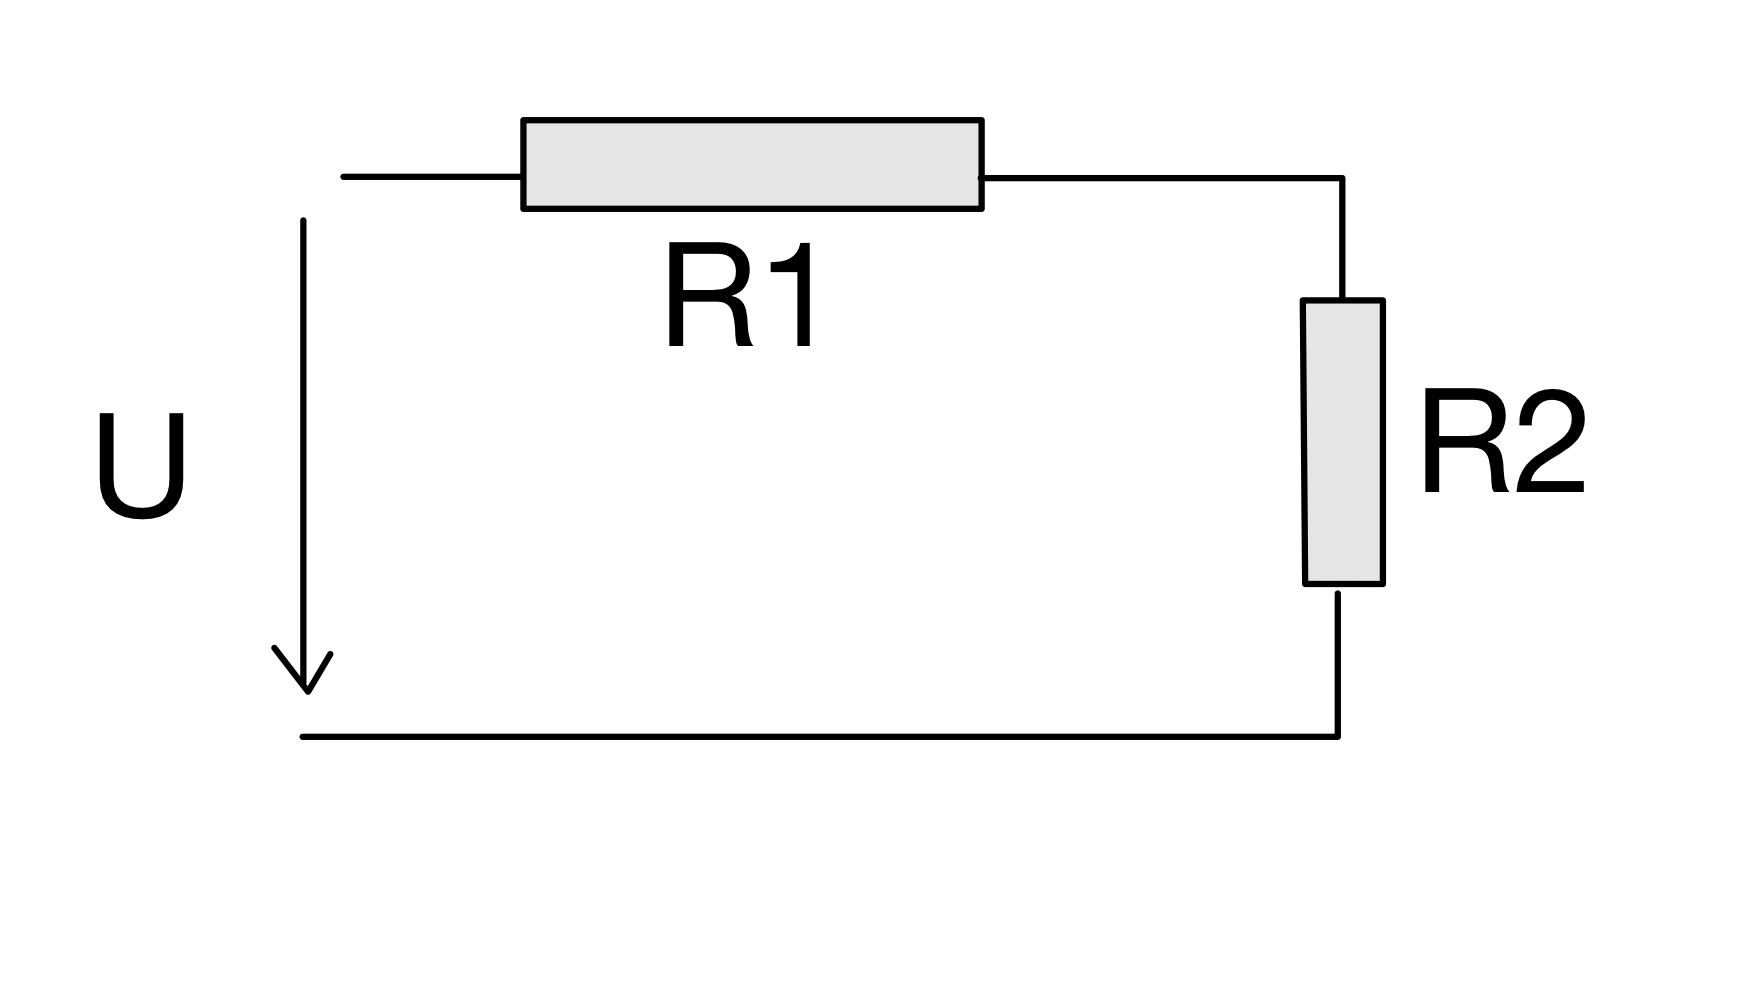
\includegraphics[width=.8\textwidth]{IMAGES/elec/divtens.jpeg}
    
\end{minipage}
\hfill
\begin{minipage}{.5\textwidth}
    En général : 
    \begin{equation}
        u_2 = u\frac{C_1}{C_1+C_2} = u\frac{R_2}{R_1+R_2}
    \end{equation}
\end{minipage}

\quad \underline{Diviseur de courant :} u constant\\
\begin{minipage}{.5\textwidth}
    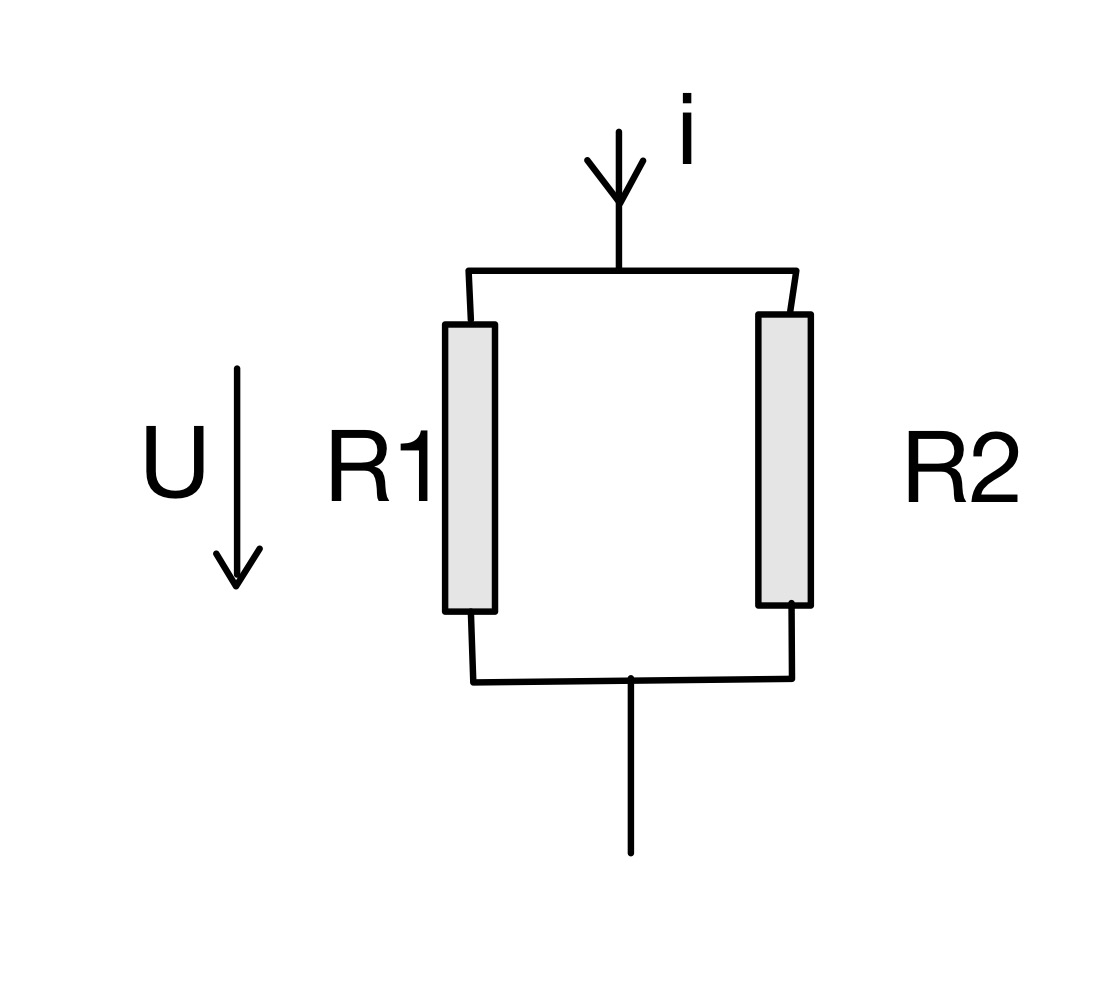
\includegraphics[width=.8\textwidth]{IMAGES/elec/divcour.jpeg}
    
\end{minipage}
\hfill
\begin{minipage}{.5\textwidth}
    En général : 
    \begin{equation}
        i_2 = i\frac{R_1}{R_1+R_2}
    \end{equation}
\end{minipage}

\quad \underline{Équivalence de sources :}\\
\begin{figure}[hbt!]
    \centering
    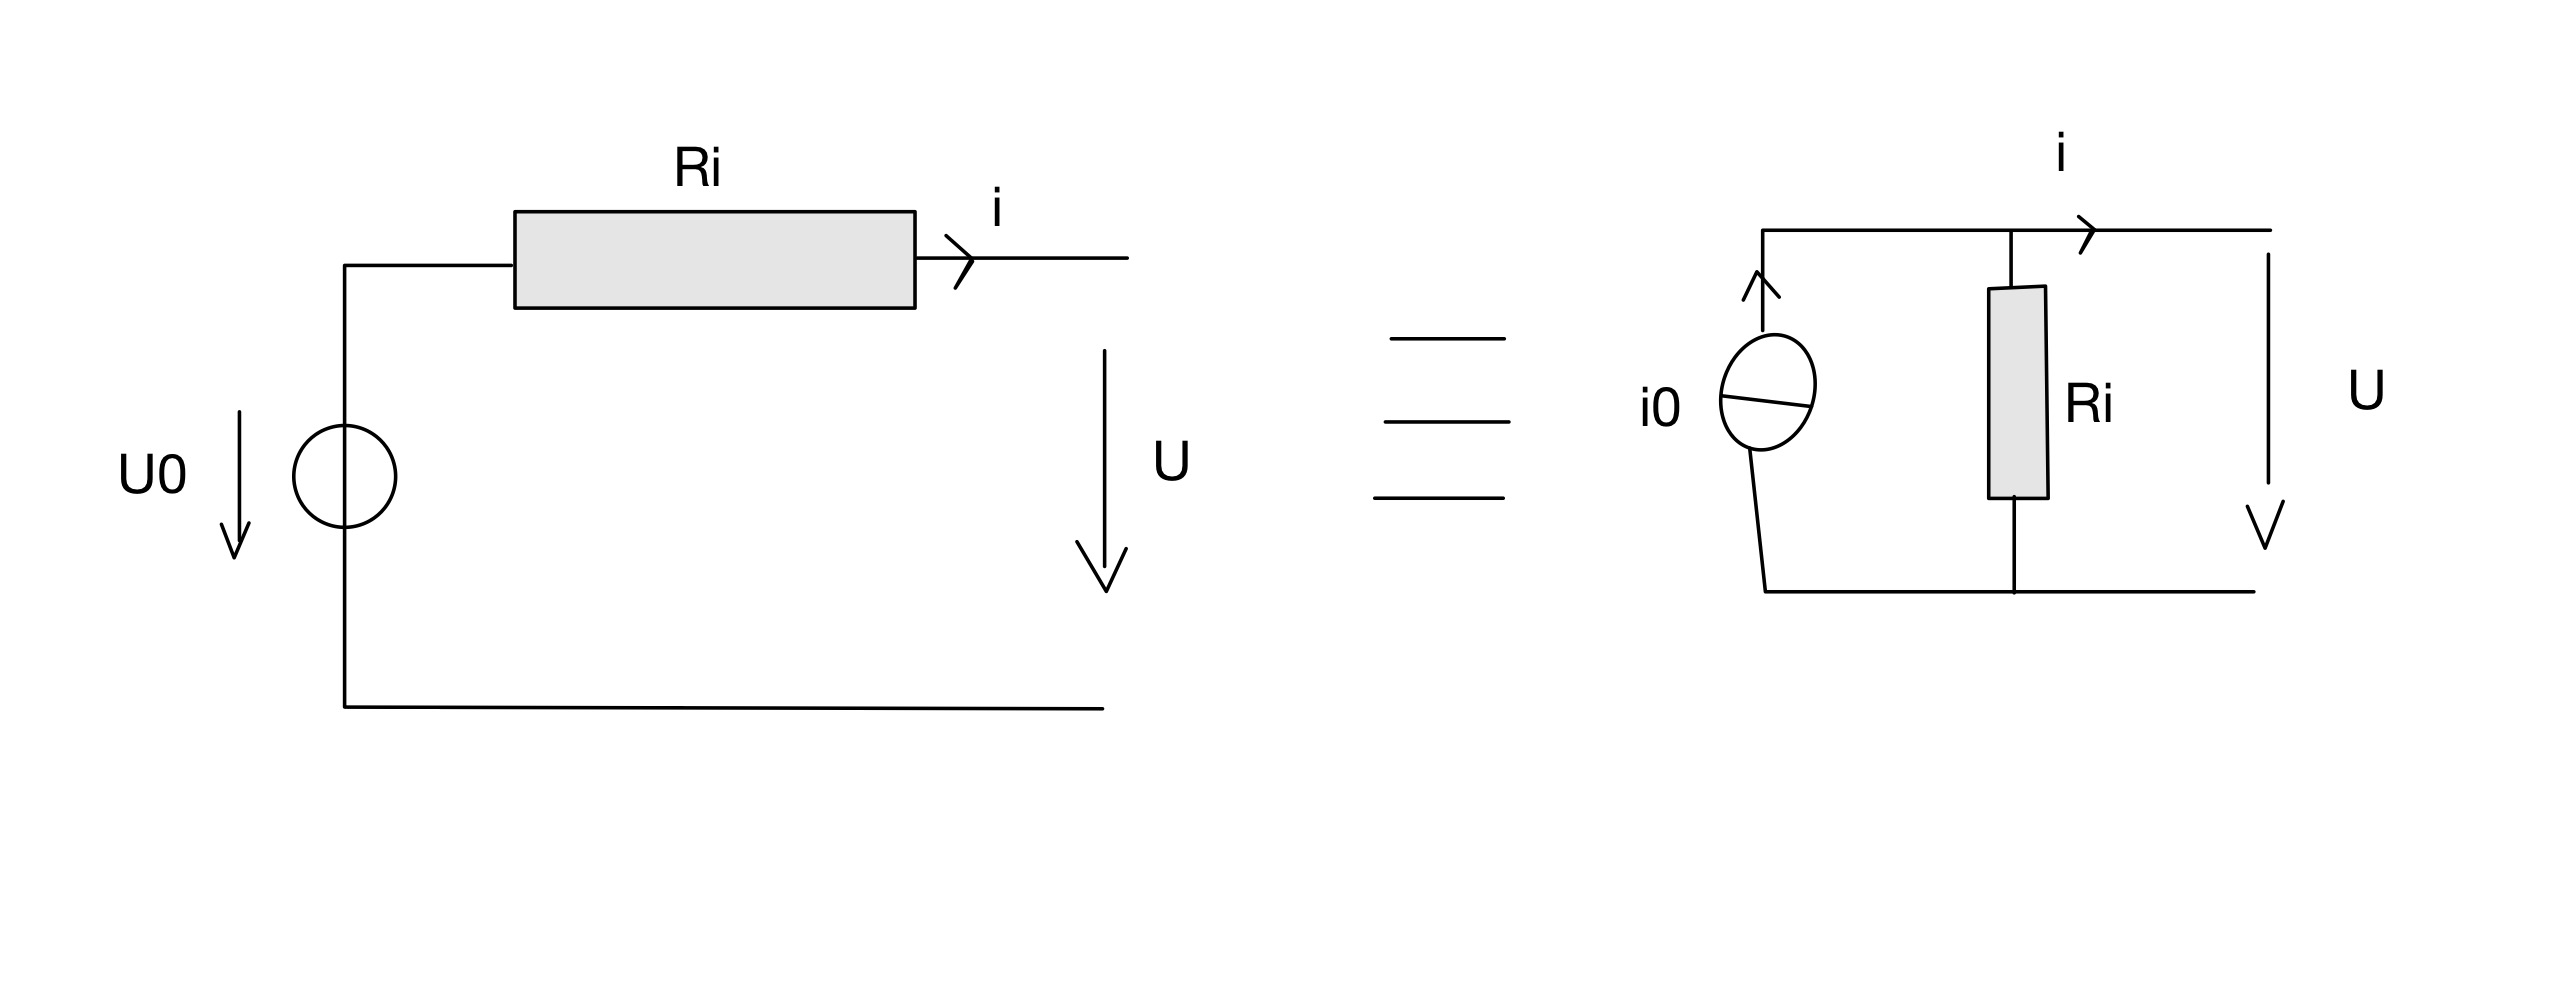
\includegraphics[width=.6\textwidth]{IMAGES/elec/eqsource.jpeg}
    
\end{figure}    
    On a ici : $i_0 = \frac{U_0}{R_i}$\\
Sources de tension et courant s'opposent et la résistance passe de série (source de tension) à parallèle (courant).

\newpage

\quad \underline{Principe superposition :}
On considère à chaque fois qu'une source et on superpose.\\
\textbf{Annuler source tension : remplacer par court-circuit}\\
\textbf{Annuler source courant : remplacer par circuit-ouvert}\\

\subsubsection{Théorème de Thévenin}
Procédure : \begin{itemize}
    \item[$\bullet$] Identifier R à étudier\\
    \item[$\bullet$] Supprimer R\\
    \item[$\bullet$] Mesurer/Calculer tensions aux bornes du circuit : tension de thévenin\\
    \item[$\bullet$] Annuler toutes les sources et déterminer R.
\end{itemize}

\subsubsection{Théorème de Norton}
Corollaire de Thévenin : remplacer un circuit complexe par un circuit avec une source de courant et R en parallèle.

\subsection{Monophasé}
\textbf{Notations :}\begin{itemize}
    \item[$\bullet$] T : période\\
    \item[$\bullet$] $\alpha$ : phase\\
    \item[$\bullet$] $f = \frac{1}{T}[H]$ fréquence\\
    \item[$\bullet$] $\omega = 2\pi f = \frac{2\pi}{T}[rad.s^{-1}$ : pulsation
\end{itemize}

\begin{equation}
    x(t) = Asin(\omega t+\alpha)
\end{equation}
Valeur moyenne : 
\begin{equation}
    \hat{X} = \frac{1}{T}\int_0^TAsin(\omega t+\alpha)dt = 0
\end{equation}
Valeur efficace :
\begin{equation}
    X=\sqrt{\frac{A^2}{T}\int_0^Tsin^2(\omega t+\alpha)dt} = \frac{A}{\sqrt{2}}
\end{equation}

\quad \underline{Puissance moyenne :}
$P_{moy} = \frac{R \hat{I}^2}{2} = R I^2$\\

\quad \underline{Valeurs crêtes :}
$\hat{U} = \sqrt{2}U$, $\hat{I} = \sqrt{2}I$
Soit : (pour I et U)
\begin{equation}
    u(t) = \sqrt{2}U cos(\omega t+\alpha)
\end{equation}

\subsubsection{Phaseurs}
$\overline{z} = a+jb$\\
Ne dépend pas du temps, représente U et I dans les complexes.\\
Le déphasage $\varphi = \alpha-\beta$ entre U et I respectivement. \\
Phaseur de crête complexe : $\hat{\overline{X}} = \sqrt{2}Xe^{i\alpha}$

\quad \underline{Dérivation :}
$\overline{Y} = (i \omega) \overline{X}$

\quad \underline{Intégration :}
$\overline{Y} = \frac{1}{i \omega} \overline{X}$\\

\textbf{Dans le domaine complexe, tous les dipôles sont les mêmes (R, inductance, capacité...)}\\
\quad \underline{Impédance :}
\begin{equation}
    \overline{Z} = \frac{\overline{U}}{\overline{I}} = Z e^{i\varphi} = R +iX [\Omega]
\end{equation}
Avec R : Résistance, X : Réactance\\
$\varphi = arctan(\frac{X}{R})$

\quad \underline{Admittance :}
\begin{equation}
    \overline{Y} = \frac{1}{\overline{Z}} = Y e^{-i\varphi} = G + iB [S]
\end{equation}
Avec G : conductance, B : susceptance\\
$\varphi = arctan(\frac{-B}{G}$



\subsubsection{Applications aux éléments}
\begin{minipage}{.3\textwidth}
    \quad \underline{Résistance :}\\
$\overline{U} = R \overline{I}$\\
$Z_R = R$, $\varphi = 0$\\
$R_R = R$, $X_R = 0$\\
$Y_R = \frac{1}{R}$, $-\varphi_R = 0$\\
$G_R = \frac{1}{R}$, $B_R = 0$\\
\end{minipage}
\vline
\begin{minipage}{.3\textwidth}
    \quad \underline{Inductance :}\\
$\overline{U} = i\omega L \overline{I}$\\
$Z_L = \omega L$, $\varphi = \frac{\pi}{2}$\\
$R_L = 0$, $X_L = \omega L$\\
$Y_L = \frac{1}{\omega L}$, $-\varphi_L = -\frac{\pi}{2}$\\
$G_L = 0$, $B_L = -\frac{1}{\omega L}$\\
\end{minipage}
\vline
\begin{minipage}{.3\textwidth}
    \quad \underline{Capacité :}\\
$\overline{U} = \frac{1}{i \omega C}\overline{I}$\\
$Z_C = \frac{1}{\omega C}$, $\varphi = -\frac{\pi}{2}$\\
$R_C = 0$, $X_C = -\frac{1}{\omega C}$\\
$Y_C = \omega C$, $-\varphi_C = \frac{\pi}{2}$\\
$G_C = 0$, $B_C = \omega C$\\
\end{minipage}

\begin{minipage}{.3\textwidth}
\quad \underline{Réseaux d'impédances :}\\
$\overline{U} = \overline{Z} \overline{I}$ : loi d'ohm généralisée\\
$\sum \overline{I_k} = 0$ : loi des noeuds\\
$\sum \overline{U_l} = 0$ : loi des mailles\\
\end{minipage}
\vline
\begin{minipage}{.3\textwidth}
\quad \underline{En série :}\\
$\overline{Z_t} = \sum \overline{Z_k}$\\
$\overline{Y_t} = \frac{1}{\sum \frac{1}{\overline{Y_k}}}$\\
\end{minipage}
\vline
\begin{minipage}{.3\textwidth}
\quad \underline{En parallèle :}\\
$\overline{Y_t} = \sum \overline{Y_k}$\\
$\overline{Z_t} = \frac{1}{\sum \frac{1}{\overline{Z_k}}}$\\
\end{minipage}

\begin{minipage}{.5\textwidth}
    \quad \underline{Diviseur de courant :}\\
$\overline{I_1} = \frac{\overline{Z_2}}{\overline{Z_1}+\overline{Z_2}}\cdot \overline{I}$\\
$\overline{I_2} = \frac{\overline{Z_1}}{\overline{Z_1}+\overline{Z_2}}\cdot \overline{I}$\\

\end{minipage}
\vline
\begin{minipage}{.5\textwidth}
    \quad \underline{Diviseur de tension :}\\
$\overline{U_1} = \frac{\overline{Z_1}}{\overline{Z_1}+\overline{Z_2}}\cdot \overline{U}$\\
$\overline{U_2} = \frac{\overline{Z_2}}{\overline{Z_1}+\overline{Z_2}}\cdot \overline{U}$\\

\end{minipage}

\subsubsection{Puissances}
\quad \underline{P active :} Valeur moyenne de puissance instantanée.
\begin{equation}
    P = UIcos(\varphi)[W]
\end{equation}
C'est l'énergie réellement convertible en travail/chaleur.\\

\quad \underline{P réactive :} Amplitude de la composante alternative de P instant.
\begin{equation}
    Q = UIsin(\varphi) [var]
\end{equation}
En [var] : volt ampère réactif. C'est une puissance fictive qui caractérise l'échange d'énergie non convertible.\\

\quad \underline{P apparente S :} Amplitude de la fluctuation de la puissance par rapport à sa valeur moyenne.
\begin{equation}
    S = UI = \sqrt{P^2+Q^2} [VA]
\end{equation}
Elle est exprimée en volt ampère.\\

\quad \underline{P complexe $\overline{S}$ :}\\
\begin{equation}
    \overline{S} = RI^2+iXI^2 = GU^2-iBU^2
\end{equation}

\quad \underline{Facteur de Puissance:}\\
\begin{equation}
    cos(\varphi) = \frac{P}{S}
\end{equation}
\textbf{Résistance : =1}, \textbf{inductance et capacité : =0}\\

\begin{minipage}{.5\textwidth}
    \quad \underline{Impédance :}\\
$P = RI^2$\\
$Q = XI^2$\\
$p(t) = P(1+cos(2\omega t+2\alpha)) + Qsin(2\omega t+2\alpha)$\\

\end{minipage}
\vline
\vline
\begin{minipage}{.5\textwidth}
    \quad \underline{Admittance :}\\
$P = GU^2$\\
$Q = -BU^2$\\
$p(t) = P(1+cos(2\omega t+2\alpha)) + Qsin(2\omega t+2\alpha)$\\

\end{minipage}



\begin{minipage}{.3\textwidth}
\quad \underline{Résistance :}\\
$P = UI = RI^2 = G8R U^2 = \frac{U^2}{R}$\\
$Q = 0$\\
$p(t) = P(1+cos(2\omega t+2\alpha))$\\

\end{minipage}
\vline
\vline
\begin{minipage}{.3\textwidth}
\quad \underline{Inductance :}\\
$P = 0$\\
$Q = UI = X_L I^2 = \omega LI^2 = -B_LU^2 = \frac{1}{\omega L} U^2 >0$\\
$p(t) = Qsin(2\omega t+2\alpha)$\\
\end{minipage}
\vline
\vline
\begin{minipage}{.3\textwidth}
\quad \underline{Capacité :}\\
$P = 0$\\
$Q = -UI = X_C I^2 = -\frac{1}{\omega C}I^2 = -B_C U^2 = -\omega CU^2<0$\\
$p(t) = Qsin(2\omega t+2\alpha)$\\
\end{minipage}


\quad \underline{Propriété d'additivité :}\\
$P_t = \sum P_j$, $Q_t = \sum Q_j$, $S_t = P_t+iQ_t$

\subsection{Triphasé}
\quad \underline{Anecdotes :}\\

\begin{itemize}
    \item[$\bullet$] Système polyphasé symétrique : il y a m phases d'ordre k(ordre de succession des phases), est un ensemble de m grandeurs sinusoïdales de même fréquence et même valeur efficace. Le déphasage entre deux valeurs consécutives : $\frac{k2\pi}{m}$\\
    \item[$\bullet$] Système direct : diagramme des phaseurs ordonné dans le sens anti-trigonométrique\\
    \item[$\bullet$] Ligne : ensemble des conducteurs transmettant l'énergie\\
    \item[$\bullet$] En triphasé : 3 conducteurs de phases (R,S,T)\\
    \item[$\bullet$]Le pôle commun aux trois sources est appelé : point neutre\\
    \item[$\bullet$] Conducteur neutre : N\\
    \item[$\bullet$] Tensions simples : les tensions prises entre neutre et conducteur de phase\\
    \item[$\bullet$] Tensions de ligne/composées : les tensions prises entre 2 conducteurs de phases (elles sont en avance de $\frac{\pi}{6}$ par rapport aux tensions simples\\
    \item[$\bullet$] Courants de lignes sont les courants traversant chaque conducteur de phase, courant de retour $ \overline{I_N} = \overline{I_R} + \overline{I_S} + \overline{I_T}$
    \item[$\bullet$] Si distance > 100km, continu meilleur car pas de puissance réactive donc moins de pertes
\end{itemize}

\quad \underline{Relations :}\\
\begin{equation}
\overline{U_{RS}} = \sqrt{3}\overline{U_{RN}}e^{i(\frac{\pi}{6})}
\end{equation}
Valable pour toutes les tensions composées : 
\begin{equation}
    U_l = \sqrt{3}U
\end{equation}
\begin{equation}
    I_{ph} = \frac{U_{ph}}{Z}
\end{equation}


\subsubsection{Étoile}
Tensions de phase se confondent avec les tensions simples : $U_{ph} = U \Rightarrow U_l = \sqrt{3}U_{ph}$ et $I_l = I_{ph} = \frac{U_{ph}}{Z}$ ainsi que $I_N = 0$\\
Si les charges sont équilibrées il n'est pas nécessaire de relier le neutre!

\subsubsection{Triangle}
Charge n'a pas de point neutre. Impédances sont alimentées par les tensions de ligne et forment un circuit fermé. \\
Les courants de phase forment un système triphasé symétrique : $I_{ph} = \frac{\sqrt{3}U}{Z}$ et les courants de lignes forment un système triphasé symétrique retardé de $\frac{\pi}{6}$ : $I_l = \sqrt{3}I_{ph}$\\
De plus : $U_{ph} = U_l = \sqrt{3} U$\\
\subsubsection{Conversion}
\textbf{Si charges équilibrées :}
\begin{equation}
    p(t) = P = 3U_{ph} I_{ph}cos(\varphi)
\end{equation}
\begin{equation}
    Q = 3U_{ph} I_{ph} sin(\varphi)
\end{equation}
\begin{equation}
    S = 3U_{ph} I_{ph} \Rightarrow \overline{S} = P+iQ = 3U_{ph}I_{ph} e^{i\varphi}
\end{equation}

\begin{table}[hbt!]
    \centering
    \begin{tabular}{|c|c|c|}
    \hline
    \multicolumn{1}{|c|}{\diagbox[width=7mm,height=5mm]{\diagbox[width=7mm,height=5mm,dir=SW]{}{}}{}} & Étoile & Triangle \\
    \hline
    $U_l$ & $\sqrt{3}U_{ph} $ & $U_{ph}$\\
    \hline
    $I_l$ & $I_{ph}$ & $\sqrt{3} I_{ph}$\\
    \hline
    $I_{ph}$ & $\frac{U_{ph}}{Z} = \frac{U_l}{\sqrt{3}Z}$ & $\frac{U_{l}}{Z}$ \\
    \hline
    P & $3 \frac{U_l^2}{Z} cos(\varphi)$ & $\frac{U_l^2}{Z}cos(\varphi)$\\
    \hline

    \end{tabular}
    \caption{Conversion Étoile/Triangle}
    
\end{table}

Entre les deux, source d'alimentation, tension, courants de lignes et P consommée ne changent pas. \\
Si charge équilibrée : $\overline{Z_{*}} = \frac{1}{3}\overline{Z_{\Delta}}$\\
Et on a : 
\begin{equation}
    \overline{Z} = \frac{\overline{Z_2} \overline{Z_{1*}}}{\overline{Z_2} + \overline{Z_{1*}}}
\end{equation}
\end{document}